\documentclass{article}
\usepackage{graphicx} 
\usepackage{multirow}
\usepackage{enumitem}
\usepackage{amssymb}
\usepackage{amsmath}
\usepackage{xcolor}
\usepackage{cancel}
\usepackage{tcolorbox}
\usepackage{physics}
\usepackage{geometry}
\usepackage{tikz}
\usepackage{tikz-3dplot}
\usepackage{pgfplots, tkz-euclide,calc}

\usetikzlibrary{angles,quotes} % for pic (angle labels)
\usetikzlibrary{arrows.meta}
\usetikzlibrary{calc}
\usetikzlibrary{decorations.markings}
\usetikzlibrary{bending} % for arrow head angle
\tikzset{>=latex} % for LaTeX arrow head
\usepackage{xcolor}
\pgfplotsset{compat=newest}

\colorlet{xcol}{blue!60!black}
\colorlet{myred}{red!80!black}
\colorlet{myblue}{blue!80!black}
\colorlet{mygreen}{green!40!black}
\colorlet{mypurple}{red!50!blue!90!black!80}
\colorlet{mydarkred}{myred!80!black}
\colorlet{mydarkblue}{myblue!80!black}
\tikzstyle{xline}=[xcol,thick,smooth]
\tikzstyle{width}=[{Latex[length=5,width=3]}-{Latex[length=5,width=3]},thick]
\tikzstyle{mydashed}=[dash pattern=on 1.7pt off 1.7pt]
\tikzset{
  traj/.style 2 args={xline,postaction={decorate},decoration={markings,
    mark=at position #1 with {\arrow{<}},
    mark=at position #2 with {\arrow{<}}}
  }
}
\def\tick#1#2{\draw[thick] (#1)++(#2:0.12) --++ (#2-180:0.24)}
\def\N{100} % number of samples
    \usetikzlibrary{patterns,snakes,shapes.arrows,3d}
    \usepgfplotslibrary{fillbetween}
	\geometry{
		total = {160mm, 237mm},
		left = 25mm,
		right = 35mm,
		top = 30mm,
		bottom = 30mm,
	}

\tikzstyle{block} = [draw, fill=white, rectangle, minimum height=3em, minimum width=6em]
\tikzstyle{sum} = [draw, fill=white, circle, node distance=1cm]
\tikzstyle{input} = [coordinate]
\tikzstyle{output} = [coordinate]
\tikzstyle{pinstyle} = [pin edge={to-,thin,black}]

\newcommand{\jawab}{\textbf{\underline{Solusi}}:}
\newcommand{\del}{\partial}
\newcommand{\cis}{\text{cis}}

\title{\textbf{Kuis 1 Permodelan Matematika}}
\author{Kelas C - Pak Kamiran}
\date{23 September 2024}

\begin{document}
    \maketitle
    \setlength{\parindent}{0pt}
    \pagenumbering{gobble}
    \begin{enumerate}
        \item Tuliskan Sistem Persamaan Diferensial dari Model yang memiliki diagram kompartemen sebagai berikut:
        \begin{center}
            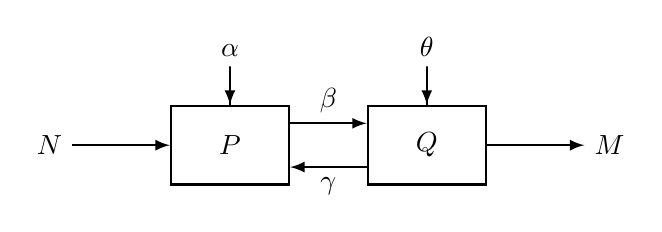
\begin{tikzpicture}[auto, node distance=2.5cm, thick, >=latex]
                % Nodes
                \node [draw, rectangle, minimum height=1cm, minimum width=1.5cm] (P) {$P$};
                \node [right of=P, draw, rectangle, minimum height=1cm, minimum width=1.5cm] (Q) {$Q$};
                
                % Arrows
                \draw[->] (P.20) -- node[above] {$\beta$} (Q.160);
                \draw[<-] (P.-20) -- node[below] {$\gamma$} (Q.-160);
                \draw[->] (P) -- ++(0, 1) node[above] {$\alpha$} -- (P);
                \draw[->] (Q) -- ++(0, 1) node[above] {$\theta$} -- (Q);
                \draw[<-] (P) -- ++(-2, 0) node[left] {$N$};
                \draw[->] (Q) -- ++(2, 0) node[right] {$M$};
            \end{tikzpicture}
        \end{center}

        \item Tentukan penyelesaian dari model dengan sistem persamaan sebagai berikut
        \[\frac{dX}{dt}=\begin{bmatrix}
            1&2&1\\
            0&1&-1\\
            0&1&2
        \end{bmatrix}\begin{pmatrix}
            x\\
            y\\
            z
        \end{pmatrix},\quad X_0=\begin{pmatrix}
            0\\
            0\\
            1
        \end{pmatrix}\]
        Sketsa grafik penyelesaiannya.

        \item Tentukan penyelesaian dan lukis diagram fasa antara $x$ dan $y$ dari model dengan sistem persamaan diferensial sebagai berikut
        \[\frac{dX}{dt}=\begin{bmatrix}
            1&-2\\
            2&1
        \end{bmatrix}\begin{pmatrix}
            x\\
            y
        \end{pmatrix},\quad\begin{pmatrix}
            x(0)\\
            y(0)
        \end{pmatrix}=\begin{pmatrix}
            2\\
            8
        \end{pmatrix}\]
    \end{enumerate}
    \jawab
    \begin{enumerate}
        \item Sistem persamaan diferensial dari model adalah sebagai berikut
        \begin{flalign}
            \frac{dP}{dt}=N+\alpha P-\beta P + \gamma Q\\
            \frac{dQ}{dt}=\beta P-\gamma Q+\theta Q-M
        \end{flalign}
        Jika diubah ke dalam bentuk matriks, maka
        \[\frac{dX}{dt}=\begin{bmatrix}
            \alpha-\beta&\gamma\\
            \beta&-\gamma+\theta
        \end{bmatrix}\begin{pmatrix}
            P\\
            Q
        \end{pmatrix}+\begin{pmatrix}
            N\\
            -M
        \end{pmatrix}\]
        \item Misalkan persamaan diatas adalah $\dot{X}=AX$, langkah pertama adalah mencari nilai eigen dari matriks $A$.
        \begin{flalign}
            \begin{vmatrix}
                1-\lambda&2&1\\
                0&1-\lambda&-1\\
                0&1&2-\lambda
            \end{vmatrix}&=0\\
            \lambda^3-4\lambda^2+3\lambda&=0\\
            \lambda(\lambda-1)(\lambda-3)&=0
        \end{flalign}
        \item 
    \end{enumerate}
\end{document}